% Source: PDF pages 2--6.
\section{Foundations}
\begin{definition}
A \textit{permutation} of size $n$ is an ordering of $1,2,\ldots,n$; for example, $123$, $321$, and so on.
\end{definition}
\begin{lemma}
There are $n!$ permutations of length $n$.
\end{lemma}
\begin{proof}
There are $n$ ways to make the first choice, then $n-1$ ways to make the next choice, and so on.
\end{proof}
\begin{definition}
A \textit{binary string} of length $n$ is an $n$-tuple made of $0$s and $1$s.
\end{definition}
\begin{example}
The binary strings of length $2$ are $00$, $01$, $10$, and $11$.
\end{example}
\begin{lemma}
There are $2^n$ binary strings of length $n$.
\end{lemma}
\begin{proof}
Every position has two choices. Making these choices in $n$ positions gives $2^n$ strings.
\end{proof}

\subsection{Bijections}
The idea is to use things we already know to define new things.
\begin{definition}
Let $A$ and $B$ be sets. A function $f\colon A\to B$ is
\begin{itemize}
\item \textit{injective} if $a\ne a'$ implies $f(a)\ne f(a')$ for all $a,a'\in A$; equivalently, $f(a)=f(a')$ implies $a=a'$;
\item \textit{surjective} if, for every $b\in B$, there is an $a\in A$ such that $f(a)=b$;
\item \textit{bijective} if it is both injective and surjective.
\end{itemize}
\end{definition}
If $A$ and $B$ are finite and in bijection, then $|A|=|B|$.
\begin{center}
\begin{tikzpicture}[>=Stealth,scale=.75]
\draw (0,0) ellipse (.4 and 1.15);
\draw (2.3,0) ellipse (.4 and 1.15);
\node at (0,1.5) {$A$}; \node at (2.3,1.5) {$B$};
\foreach \y in {-.75,-.25,.25,.75}{
  \fill (0,\y) circle (1.7pt); \fill (2.3,\y) circle (1.7pt);
  \draw[->] (.2,\y)--(2.1,\y);
}
\end{tikzpicture}
\end{center}

A well-defined function $f\colon A\to B$ is a bijection if and only if there is a function $g\colon B\to A$ such that
\[
f(g(b))=b\quad(b\in B),\qquad g(f(a))=a\quad(a\in A).
\]
Here $g$ is the \textit{inverse} of $f$. The first identity gives surjectivity of $f$ and the second gives injectivity.
% The handwritten injective/surjective annotations above these identities
% are reversed; the implications are corrected here.
To prove that $f$ is a bijection, we can either
\begin{enumerate}
\item show that it is injective and surjective, or
\item find its inverse.
\end{enumerate}

\subsection{Subsets}
\begin{definition}
A \textit{subset} of $[n]=\{1,\ldots,n\}$ is a collection of some elements of $[n]$, possibly empty. The only subset of $[0]=\varnothing$ is $\varnothing$, the empty set.
\end{definition}
\begin{lemma}
For $n\in\N$, there are $2^n$ subsets of $[n]$.
\end{lemma}
\begin{proof}
Every element is either picked or not picked, giving $2^n$ choices.
\end{proof}
\begin{proof}[Bijective proof]
Fix $n$. Let $A$ be the set of subsets of $[n]$, and let $B$ be the set of binary strings of length $n$. Define $f\colon A\to B$ by
\[
f(S)=\sigma_1\sigma_2\cdots\sigma_n,
\qquad
\sigma_i=\begin{cases}0,&i\notin S,\\1,&i\in S.\end{cases}
\]
We need to show that $f$ is well-defined, injective, and surjective.
\begin{enumerate}
\item For $S\in A$, the string $f(S)$ always has length $n$ and every entry is $0$ or $1$, so $f(S)\in B$.
\item If $f(S)=f(T)$, then $i\in S$ if and only if $i\in T$, so $S=T$.
\item Given $\sigma_1\cdots\sigma_n\in B$, let $S=\{i:\sigma_i=1\}$. Then $S\in A$ and $f(S)=\sigma_1\cdots\sigma_n$ by definition.
\end{enumerate}
Thus $|A|=|B|=2^n$.
\end{proof}
\begin{lemma}
There are $\displaystyle\binom{n}{k}=\frac{n!}{k!(n-k)!}$ subsets of $[n]$ with $k$ elements, for $n\in\N$ and $0\le k\le n$.
\end{lemma}
\begin{proof}
There are
\[
n(n-1)(n-2)\cdots(n-k+1)=\frac{n!}{(n-k)!}
\]
ways to choose a tuple of length $k$ using distinct elements of $[n]$. A subset of size $k$ is such a tuple with the order disregarded. Since there are $k!$ ways to order its elements, there are
\[
\frac{1}{k!}\frac{n!}{(n-k)!}=\binom{n}{k}
\]
subsets of $[n]$ of size $k$.
\end{proof}

\Needspace{8\baselineskip}
\subsection{Multisets}
\begin{definition}
A \textit{multiset} of size $n$ with $t$ types is a collection of $n$ elements in $\{1,\ldots,t\}$ in which elements can repeat. Equivalently, it is a sequence $(m_1,\ldots,m_t)\in\N^t$ with $m_1+\cdots+m_t=n$.
\end{definition}
The two descriptions are related by letting $m_i$ be the number of elements of type $i$. Here, and throughout these notes, $0\in\N$.
\begin{theorem}
For $n,t\in\N$ and $t\ge1$, there are $\displaystyle\binom{n+t-1}{t-1}$ multisets of size $n$ with $t$ types.
\end{theorem}
\begin{proof}[Idea of proof]
For example, $m_1+m_2+m_3=5$ with $(m_1,m_2,m_3)=(1,2,2)$ can be represented by five balls and two dividing lines.
\begin{center}
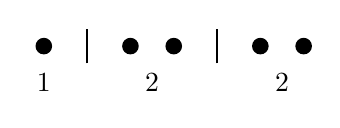
\begin{tikzpicture}[x=.55cm,y=.55cm]
\foreach \x in {0,2,3,5,6}{\fill (\x,0) circle (3pt);}
\foreach \x in {1,4}{\draw[thick] (\x,-.4)--(\x,.4);}
\node[below] at (0,-.4) {$1$};
\node[below] at (2.5,-.4) {$2$};
\node[below] at (5.5,-.4) {$2$};
\end{tikzpicture}
\end{center}

We can move the lines around. In general, we have $n$ balls and $t-1$ lines to divide them. Choose the $t-1$ positions for the lines among $n+t-1$ positions, giving $\displaystyle\binom{n+t-1}{t-1}$ possibilities.
\end{proof}

\subsection{Combinatorial proofs}
Bijections can give \textit{combinatorial proofs} of identities $\mathrm{LHS}=\mathrm{RHS}$:
\begin{enumerate}
\item Find sets $A$ and $B$ such that $\mathrm{LHS}=|A|$ and $\mathrm{RHS}=|B|$.
\item Prove that $A$ and $B$ are in bijection.
\item Conclude that $\mathrm{LHS}=|A|=|B|=\mathrm{RHS}$.
\end{enumerate}
A special case is to count one set in two ways.
\begin{example}
Give a combinatorial proof that $\displaystyle\binom{n}{k}=\binom{n}{n-k}$ for $n,k\in\N$ and $0\le k\le n$.
\end{example}
\begin{proof}
Let
\[
A=\{\text{subsets of $[n]$ of size $k$}\},\qquad
B=\{\text{subsets of $[n]$ of size $n-k$}\}.
\]
Then $|A|=\binom{n}{k}$ and $|B|=\binom{n}{n-k}$. Define $f\colon A\to B$ by $f(S)=[n]\setminus S$, the complement of $S$ in $[n]$.
\begin{enumerate}
\item If $|S|=k$, then $|f(S)|=|[n]\setminus S|=n-k$, so $f$ is well-defined.
\item Taking the complement twice gives $[n]\setminus([n]\setminus S)=S$, so the same complement operation is the inverse.
\end{enumerate}
Thus $f$ is a bijection and $\binom{n}{k}=|A|=|B|=\binom{n}{n-k}$.
\end{proof}
\begin{example}
Prove that $\displaystyle 2^n=\sum_{k=0}^n\binom{n}{k}$.
\end{example}
\begin{proof}
Let $A$ be the set of all subsets of $[n]$, so $|A|=2^n$. Write $A$ as the disjoint union
\[
A=A_0\cup A_1\cup\cdots\cup A_n,
\qquad A_k=\{\text{subsets of $[n]$ of size $k$}\}.
\]
Disjointness ensures that no subset is counted twice. Therefore
\[
\begin{aligned}
2^n&=|A|\\
&=\left|\bigcup_{k=0}^n A_k\right|\\
&=\sum_{k=0}^n|A_k|\\
&=\sum_{k=0}^n\binom{n}{k}.
\end{aligned}
\]
\end{proof}
Common objects in combinatorial proofs include subsets, permutations, binary strings, multisets, and lattice paths.
\begin{definition}
A \textit{lattice path} is a sequence of steps that starts and ends at specified points in $\Z^d$.
\end{definition}
\begin{example}
Find the number of lattice paths in $\Z^2$ that start at $(0,0)$ and end at $(a,b)\in\N^2$, using the steps $N=(0,1)$ and $E=(1,0)$.\par\medskip
A walk ending at $(a,b)$ must have $a$ east steps and $b$ north steps, for a total of $a+b$ steps. Choose the $a$ east-step positions; the remaining steps are uniquely determined. Hence there are $\displaystyle\binom{a+b}{a}$ paths.
\end{example}
